\documentclass[15pt, a5paper]{article}
\usepackage{amsfonts} % Package
% \usepackage{amsfonts,amsmath,amssymb}
\usepackage[margin=1in]{geometry}
\usepackage{graphicx}
\usepackage{float}
\def \eqn{y=\frac{x}{3x^2-2x+3}} % Macros
\begin{document}
\textbf{Notations: }\\

\begin{figure}[H]
    \centering
    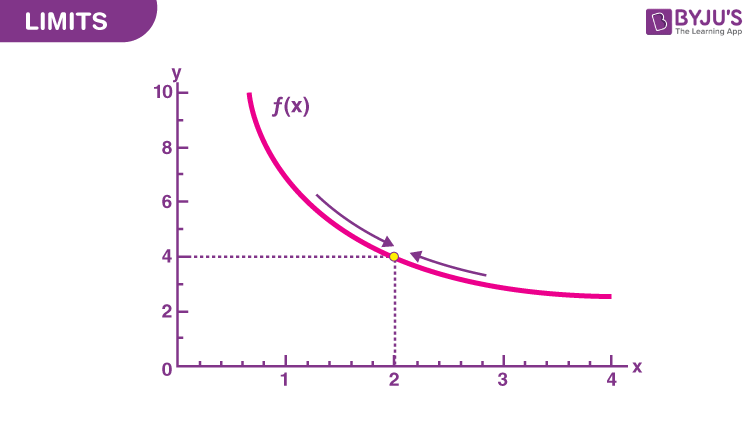
\includegraphics[width=0.5\linewidth]{Limits.png}\\
    \caption{This is a visual of Limit}
\end{figure}

\begin{enumerate}
    \item The Equation is $\eqn$.
    \item The Mathematical Notation for the set of all Real Numbers is: $\mathbb{R}$
    \item The Mathematical Notation for the set of Integers is: $\mathbb{Z}$
    \item The Mathematical Notation for the set of Rational Numbers is: $\mathbb{Q}$
    \item The Equation is $\eqn$.
\end{enumerate}
\end{document}
